\documentclass[11pt]{article}
\usepackage{graphicx} % Required for inserting images
\usepackage{tabularx}
\usepackage{changepage}
\usepackage{pgfplots}
\usepackage{amsmath}
\usepackage{graphicx}
\usepackage{caption}  % Required for \captionof command
\usepackage{hyperref}
\usepackage[a4paper,
            left=0.6in,
            top=1.0in,
            right=0.6in]{geometry}

\title{Networked software for distributed systems\\Project 5}
\date{2022-2023}

\begin{document}

\begin{titlepage}
\begin{center}
		\begin{figure}[ht]
			\centering\includegraphics[width=0.7\textwidth]{resources/Logo_Politecnico_Milano.png}
		\end{figure}
        
        \vspace{3.5cm}

        \LARGE
        \textit{Networked software for distributed systems}\\

        \vspace{0.5cm}
        \Large
        \textbf{Environmental Monitoring using IoT Devices }
        
        \vspace{\fill}
  
		\large
		\begin{tabularx}{\linewidth}{@{}lXl@{}}
			\textit{Authors:}  & & \textit{Professors:} \\
			Stefano Carraro      & & Prof.\@ Luca Mottola\\
			Stefano Fossati  & & Prof. Alessandro Margara \\
			Andrea Restelli & & \\
		\end{tabularx}		
		\thispagestyle{empty}

        \vspace{1cm}

        2022-2023
           
\end{center}
\end{titlepage}

\tableofcontents
\cleardoublepage

%%%
\section{Introduction}

\subsection{Request}
\subsubsection{Description}
In this project, you have to implement a program that analyzes open datasets to study the evolution of the COVID-19 situation worldwide. The program starts from the dataset of new reported cases for each country daily and computes the following queries:
\begin{itemize}
  \item Seven days moving average of new reported cases, for each county and for each day
  \item Percentage increase (with respect to the day before) of the seven days moving average, for each country and for each day
  \item Top 10 countries with the highest percentage increase of the seven days moving average, for each day
\end{itemize}
You can either use real open datasets or synthetic data generated with the simulator developed for Project \#4.

A performance analysis of the proposed solution is appreciated (but not mandatory). In particular, we are interested in studies that evaluate (1) how the execution time changes when increasing the size of the dataset and/or number of countries; (2) how the execution time decreases when adding more processing cores/hosts. 

\subsubsection{Assumption and Guidelines}
\begin{itemize}
    \item When using a real dataset, for countries that provide weekly reports, you can assume that the weekly increment is evenly spread across the day of the week.
\end{itemize}


\subsubsection{Technologies}
Apache Spark or MPI

\subsection{Additional Assumptions}
\begin{itemize}
    \item Since the seven days moving average is calculated by summing up the values of the past seven days and dividing by seven, it is necessary to have a complete set of data for accurate calculation. Therefore, for the initial six days, the average is based on the available records, and as each subsequent day's data becomes available, it is incorporated into the calculation, resulting in a more accurate representation of the trend.
\end{itemize}

\section{Project analysis and considerations}
The objective of this project is to analyze a static dataset by executing three queries sequentially while leveraging the computational power of multiple cores/hosts for enhanced performance. In such a scenario, Spark emerges as an ideal solution, with its Spark SQL API offering a comprehensive range of functionalities to effectively address the project requirements. Notable advantages provided by the Spark SQL API include:
\begin{itemize}
    \item seamless handling of CSV datasets through dataframes
    \item built-in windowing functions that facilitate data aggregation over specified time periods
    \item efficient and transparent distribution of computational tasks across multiple worker nodes
\end{itemize}
These features make Spark SQL an excellent framework for tackling the project requirements.


\section{Design and Implementation}

\subsection{Input reading and preprocessing}
The program reads the input dataset from csv files with two possible structures. 
The first type is that of a real dataset by European Center for Disease Prevention(ECDC), available \href{https://www.ecdc.europa.eu/en/publications-data/download-todays-data-geographic-distribution-covid-19-cases-worldwide}{here}. The file contains records of daily cases of COVID-19 for each country in the world from 31/12/2019 to 14/12/2020. Here below is the header of the csv file (last columns have been abbreviated for readability).

\begin{center}
\scriptsize % Reduce font size
\begin{tabular}{|c|c|c|c|c|c|c|c|c|c|c|c|}
  \hline
  \textbf{dateRep} & \textbf{day} & \textbf{month} & \textbf{year} & \textbf{cases} & \textbf{deaths} & \textbf{country} & \textbf{geoId} & \textbf{cCode} & \textbf{pop2019} & \textbf{cExp} & \textbf{cum} \\
  \hline
\end{tabular}
\end{center}

The second type of supported dataset is that produced by the simulator developed in Project \#4. Being simulated data, dates are here simply days starting from day 1, while countries are represented by integer country ids.
Here below is the header of this second type of csv file:

\begin{center}
\scriptsize % Reduce font size
\begin{tabular}{|c|c|c|c|c|}
  \hline
  \textbf{day} & \textbf{country\_id} & \textbf{non\_infected} & \textbf{infected} & \textbf{immune} \\
  \hline
\end{tabular}
\end{center}

Both the types of csv files are preprocessed and reduced to a common structure of the dataset, where only interesting columns are maintained.
To do so we exploited two different implementations of the same abstract class \texttt{AbstractPreprocessor}, \texttt{EcdcPreprocessor} for the real dataset and \texttt{SyntheticDataPreprocessor} for synthetic data generated by the simulator.

\begin{center}
    \includegraphics[width=0.6\textwidth]{preprocessor.png}
    \captionof{figure}{The two input preprocessors.}
    \label{fig:preprocessor}
\end{center}

The resulting dataset has the following common structure, that is then used for the three queries.

\begin{center}
\scriptsize % Reduce font size
\begin{tabular}{|c|c|c|}
  \hline
  \textbf{date} & \textbf{cases} & \textbf{country} \\
  \hline
  ... & ... & ... \\
  \hline
\end{tabular}
\end{center}

\subsection{Data analysis}
The project requires to compute three queries on the dataset.
\subsubsection{Seven days moving average}
Grouping the dataset by country, we exploited the built-in Spark SQL \textit{Window} functions to consider, for each day, the previous seven days and collect the sum of the new cases over this period. With a slide of 1 day, then we compute:

\begin{equation*}
    \text{MA} = \frac{{\sum_{i=1}^{7} new\_cases\_i}}{7}
\end{equation*}

\subsubsection{Percentage increase of the MA}
To compute this query we exploited again the \textit{Window} functions considering, for each day, the seven days MA of the day before:

\begin{equation*}
    \text{Percentage Increase} = \left( \frac{{\text{MA}_\text{current day} - \text{MA}_\text{previous day}}}{{\text{MA}_\text{previous day}}} \right) \times 100
\end{equation*}

\subsubsection{Top 10 countries with the highest percentage increase}
Finally, to compute, for each day, the top 10 countries with the highest percentage increase, we ordered the countries by decreasing percentage increase and took the first 10 records. In this way, even in case of ties, we are sure to keep 10 and only 10 countries for each day.

\subsection{Caching}
Since each of the last two queries were based on the results of the previous one (percentage increase of the moving average and top 10 countries with the highest percentage increase), the caching capabilities offered by Spark perfectly fitted our needs. For this reason, after each query, the results are cached to be used in the following one without recomputing the whole results from scratch. Furthermore, after the computation of the second query, the results of the first are unpersisted, and the same is done for the results of the second query after those of the third query have been computed.

\begin{center}
    \includegraphics[width=0.8\textwidth]{caching.png}
    \captionof{figure}{A diagram of the caching strategy}
    \label{fig:caching}
\end{center}

\subsection{Writing to file}
To write the results of the computed queries on file, we had to collect the DataFrame to a single partition by using \textit{coalesce(1)}, and then write it to a CSV file. Without doing so, each partition would have written its own file, resulting in multiple files to be manually merged.

\section{Performance analysis}
In this section we analyze how the \textit{execution time} varies with respect to:
\begin{itemize}
    \item the size of the dataset and/or number of countries
    \item the number of processing cores/hosts
\end{itemize}

\subsection{Changing the size of the dataset}
To change the size of the dataset we have two possibilities:
\begin{itemize}
    \item change the number of days records are available
    \item change the number of countries records are available
\end{itemize}

We applied these transformations both to the ECDC real dataset and to the synthetic dataset generated by the simulator, obtaining datasets with 50, 100, 150, ..., 350 days, and 50, 100, 150, 200 countries. The experiments were run using a single worker on a single physical machine, monitoring the execution time from the Spark history server. The results presented in Tables \ref{tab:dates} and \ref{tab:countries} highlight the relationship between the size of the dataset and the corresponding execution time. It can be observed that as the dataset size increases, the execution time also increases, exhibiting an almost linear relationship. This suggests that larger datasets require more time for processing and analysis.

\begin{table}[htbp]
\begin{minipage}{0.5\textwidth}
  \centering
  \caption{Varying the number of days}
  \label{tab:dates}
  \begin{tabular}{|c|c|}
    \hline
    \textbf{Day} & \textbf{Execution Time} \\
    \hline
    50 & 24s \\
    100 & 31s \\
    150 & 32s \\
    200 & 35s \\
    250 & 36s \\
    300 & 37s \\
    350 & 45s \\
    \hline
  \end{tabular}
\end{minipage}%
\begin{minipage}{0.5\textwidth}
  \centering
  \caption{Varying the number of countries}
  \label{tab:countries}
  \begin{tabular}{|c|c|}
    \hline
    \textbf{Countries} & \textbf{Execution time} \\
    \hline
    50 & 31s \\
    100 & 34s \\
    150 & 38s \\
    200 & 39s \\
    \hline
  \end{tabular}
\end{minipage}
\end{table}

\begin{figure}[h]
    \centering
    \begin{minipage}{0.45\textwidth}
      \centering
      \caption{Varying the number of dates}
      \label{fig:dates}
      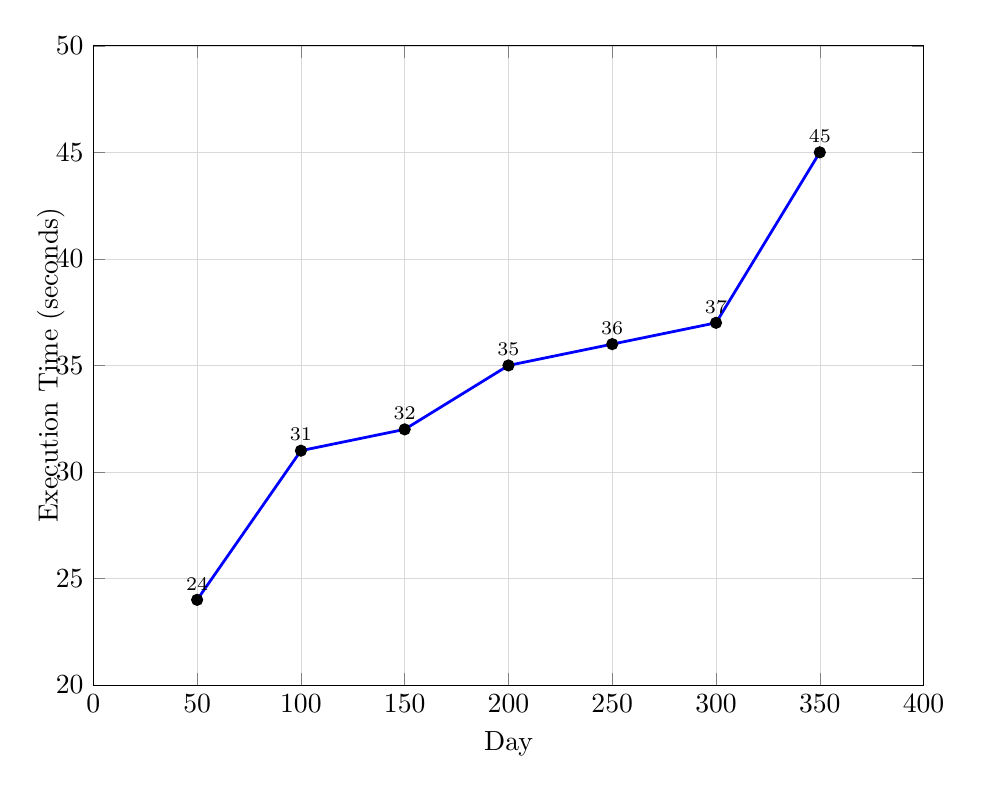
\begin{tikzpicture}
        \begin{axis}[
            xlabel={Day},
            ylabel={Execution Time (seconds)},
            xmin=0, xmax=400,
            ymin=20, ymax=50,
            grid=both,
            grid style={line width=0.2pt, draw=gray!30},
            width=\textwidth,
            height=0.8\textwidth,
            mark=none,
            ylabel style={yshift=-10pt}
          ]
          \addplot[
            scatter,
            only marks,
            mark=*,
            nodes near coords,
            point meta=explicit symbolic,
            every node near coord/.append style={anchor=south, font=\scriptsize},
          ] table[meta index=2] {
          x     y     label
          50    24   24 
          100   31   31
          150   32   32
          200   35   35
          250   36   36
          300   37   37
          350   45   45
        };
        \addplot[
            line width=1pt,
            color=blue,
            mark=none,
          ] table {
          x     y
          50    24
          100   31
          150   32
          200   35
          250   36
          300   37
          350   45
        };
      \end{axis}
      \end{tikzpicture}
    \end{minipage}
     \begin{minipage}{0.45\textwidth}
      \centering
      \caption{Varying the number of countries}
      \label{fig:countries}
      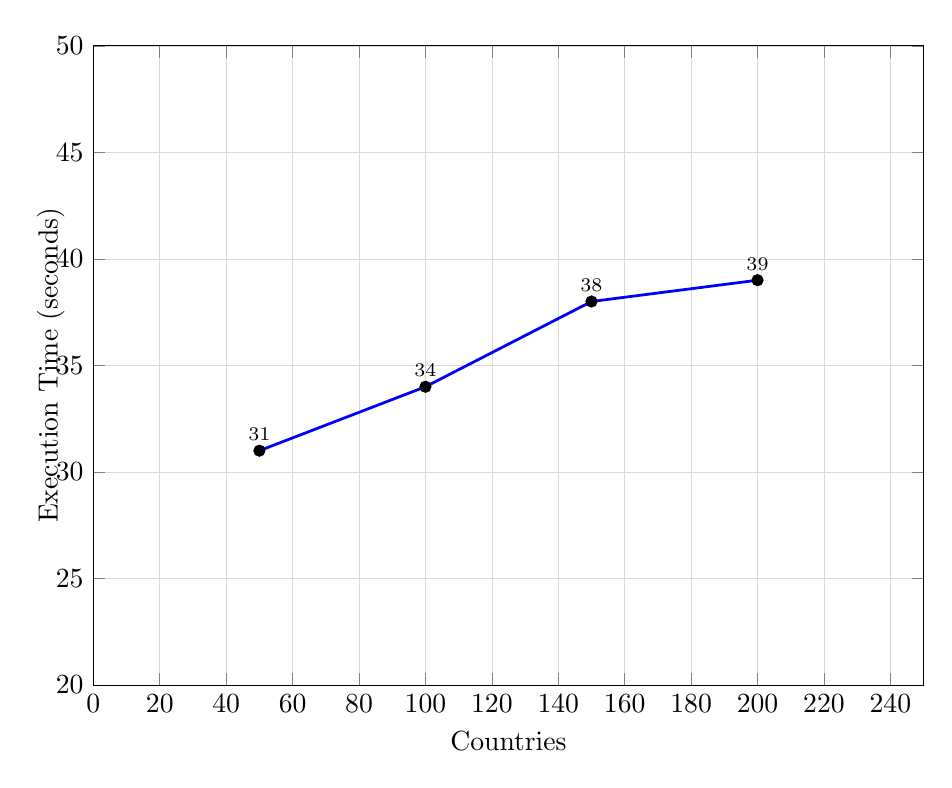
\begin{tikzpicture}
        \begin{axis}[
            xlabel={Countries},
            ylabel={Execution Time (seconds)},
            xmin=0, xmax=250,
            ymin=20, ymax=50,
            grid=both,
            grid style={line width=0.2pt, draw=gray!30},
            width=\textwidth,
            height=0.8\textwidth,
            mark=none,
            ylabel style={yshift=-10pt}
          ]
          \addplot[
            scatter,
            only marks,
            mark=*,
            nodes near coords,
            point meta=explicit symbolic,
            every node near coord/.append style={anchor=south, font=\scriptsize},
          ] table[meta index=2] {
          x     y     label
          50    31    31
          100   34    34
          150   38    38
          200   39    39
        };
        \addplot[
            line width=1pt,
            color=blue,
            mark=none,
          ] table {
          x     y
          50    31
          100   34
          150   38
          200   39
        };
      \end{axis}
      \end{tikzpicture}
    \end{minipage}
\end{figure}

\subsection{Changing the number of workers}
To carry out this second analysis we considered the full ECDC dataset, increasing the number of worker hosts from 1 to 3 and monitoring the execution time from the Spark history server. The results are presented in Figure \ref{fig:workers}. 

As expected, we observed a decrease in the execution time as the number of available workers increased. However, the performance improvement was not as significant as initially expected, potentially due to the dataset size, which may not be large enough to fully utilize the additional computational power offered by the extra workers. To verify this claim we performed the computation with an augmented dataset obtained by the simulator of Project \#3, but the results were similar. Another factor affecting the performance boost is the increase of latency caused by the introduction of more workers in the computation.

\begin{figure}[h]
    \centering
    \caption{Varying the number of workers}
    \label{fig:workers}
    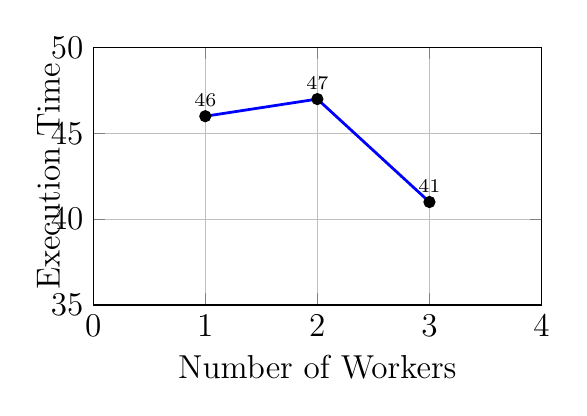
\begin{tikzpicture}
      \begin{axis}[
          xlabel={Number of Workers},
          ylabel={Execution Time},
          xmin=0, xmax=4,
          ymin=35, ymax=50,
          grid=both,
          grid style={line width=0.2pt, draw=gray!50},
          width=0.6\textwidth, % Adjusted width
          height=0.4\textwidth, % Adjusted height
          mark=none,
          font=\large, % Adjust font size
          ylabel style={yshift=-10pt}, % Reduce space between y-axis description and plot
        ]
        \addplot[
            scatter,
            only marks,
            mark=*,
            nodes near coords,
            point meta=explicit symbolic,
            every node near coord/.append style={anchor=south, font=\scriptsize},
          ] table[meta index=2] {
          x     y     label
          1     46   46
          2     47   47
          3     41   41
        };
        \addplot[
            line width=1pt,
            color=blue,
            mark=none,
          ] table {
          x     y
          1     46
          2     47
          3     41
        };
      \end{axis}
    \end{tikzpicture}
\end{figure}

\end{document}
